%!TEX root = ../main.tex
% Chapter Template



\chapter{Introduction} % Main chapter title
\label{ch:Introduction} % Change X to a consecutive number; for referencing this chapter elsewhere, use \ref{ChapterX}

%----------------------------------------------------------------------------------------
%	SECTION 1
%----------------------------------------------------------------------------------------\section{Personal Statement}
% Alice: "I've implemented a system that tolerates the presence of any attacker"\\
% % Bob: "Which attacker?"\\
% % Alice: "A trivial attacker; one that does nothing."\\
% Bob: "What does your system do?"\\
% Alice: "Nothing"\\
% Bob: "Oh! That I can believe."\\

% \todo[inline]{TOO GENERAL}
% A \emph{secure system} preserves its integrity, confidentiality and availability in the presence of adversaries~\cite{CIAModel}. 
% %A \emph{robust system} preserves its integrity in the presence of adversaries.
% Not all adversaries are the same; a passive attacker only observes, and while this attacker may not compromise the integrity or the availability of the system, they may compromise its confidentiality. 

% %What does it mean for a system to work in the presence of an adversary?
% \begin{itemize}
%     \item There have been not many uses for coalgebra and security.
%     \item Noninterference is a behavioural property 
% \end{itemize}

% Modern systems must not only be correct, but also secure. Proving that a system is correct is a difficult problem, but I would say that proving that a system is secure is exponentially more difficult. Correctness proofs study properties of the system in isolation or under strong interaction guarantees, i.e., the environment never misbehaves. 
\section{Motivation: Classifying Attackers} 
To protect our systems, we need to understand what attackers can do to them. Basin and Cremers~\cite{KnowYourEnemy} quantify the power attackers in security protocols by defining a security protocol hierarchy with respect to a fixed security property and a set of attacker models. %introduced \emph{Scyther}~\cite{Scyther}.
The position of a protocol in the hierarchy depends on its level of assurance with respect to the confidentiality property that the attackers aim to break: the protocols higher in the hierarchy can tolerate the presence of more powerful attackers (i.e., attackers with more capabilities). More precisely, the protocol hierarchy with respect to a property $P$ is a directed acyclic graph whose nodes are pairs of a protocol $\Pi$ and set of attacker capabilities $K$; there is an edge from a node $(\Pi_1,K_1)$ to a node $(\Pi_2,K_2)$ if $\Pi_1$ satisfies the property $P$ in the presence of an attacker with capabilities $K_1$, but adding additional capabilities to the attacker would break the property $P$ in the protocol $\Pi_1$, whilst the property $P$ is still satisfied in the protocol $\Pi_2$ despite the addition of those capabilities.

To check if a protocol satisfies a confidentiality property in the presence of adversaries, Basin and Cremers model the protocol as symbolic transition system, and they model an adversary as a set of compromise rules that enable previously inexistent transitions in the protocol. These new transitions expand the set of reachable states, which now may contain a state where the knowledge of the attacker has enough sensitive information to break the property being verified. The idea of an attacker adding new transitions to an existing system is simple yet powerful, because it allows us to study exceptional behaviours of the system. However, to which extend can an attacker add new transitions to a system? Can they add arbitrary transitions? Can they also remove existing transitions? All these are pertinent questions, and their answers have interesting implications. Basin and Cremers do not allow attackers to create arbitrary transitions; instead, attackers can only create these transitions based on the compromise rules that are available to them. These compromise rules span over the following three aspects: \emph{which} kind of data is compromised, \emph{whose} data is it, and \emph{when} the compromise occurs. 

The attackers described by Basin and Cremers use symbolic compromise rules that abstract the concrete implementation of attacks and focus exclusively on their effects. More precisely, a transition generated by a compromise rule changes the state of the knowledge of the attacker (e.g. the attacker now knows the long term keys). Since these transitions are symbolic, we do not know how the attacker may concretely obtain such data; we simply assume that they can and that they do. %The semantics of a new transition $a\rightarrow b$ introduced by attackers corresponds to an abstraction of the effect of some attack at the source state $a$ which causes the system to reach a state $b$. 
%In this sense, the attacker has capabilities to change the state of the system. 
While arbitrary transitions are theoretically possible, they may be practically infeasible since it is impossible to create secure systems against arbitrary state changes. For example, an attacker could, in theory, create a transition from a state where they have no knowledge about any secrets to a state where they have knowledge of all of the secrets. Such attacker could clearly break any confidentiality protocol, but the realism of such attacker model is questionable. 

\section{Beyond Confidentiality and Symbolic Attackers}
The work by Basin and Cremers verifies protocols with respect to confidentiality properties, but more precisely with respect to \emph{safety} properties, since it uses a reachability approach. It is possible to study similar safety properties using their method, even if the properties address domains beyond confidentiality, i.e., integrity or availability. We are particularly interested in studying the \emph{robustness} of systems, a concept which is closer to integrity than it is to confidentiality. 
%Robustness is a property related to the integrity of systems in the presence of adversaries. 

Informally, a \emph{robust system} preserves its integrity in the presence of adversaries: despite the effect of attacks, the system does not reach any critical states. %If we are to use a method similar to the one shown by Basin and Cremers, we need to define attacker models in such a way that these attackers enable new transitions. 
We are interested both in quantifying how robust a system is and also in the concrete strategies that attackers use when attacking the system. Since Basin and Cremers describe attackers with symbolic capabilities, 
%(e.g., an attacker can reveal a long-term secret key); this simplifies the verification process, 
the details of how information is revealed to attackers are abstracted away. %Unfortunately, due to this high level of abstraction, we do not learn how an attacker can actually obtain those secrets.  
To learn how attackers may compromise robustness, we are going to lower the level of abstraction of attackers: we define attackers as sets of concrete actions (e.g., the attacker replaces the value of a variable $x$ by its complement) instead of a set of symbolic transition rules (e.g., the attacker learns the short-term secret keys). We formalise the actions of the attacker using {spatial transformations}. A \emph{spatial transformation} is an endofunction in the set of states of a transition system; i.e. it is a function that maps states to states.%Under this formulation, attackers correspond to sets of \emph{spatial transformations}. 

\section{Idea: Attackers as Sets of Spatial Transformations}
%We now give an idea of how the the compromise rules of attackers in~\cite{KnowYourEnemy} can be generalised to spatial transformations. 
We now illustrate the effects of a spatial transformation in the behaviour of a transition system: consider the set of integer number pairs $\Z\times\Z$ and the transition function $\delta\colon \Z\times\Z\rightarrow \Z\times\Z$ that maps $(x,y)\in \Z$ to $(x^2,y)$. The pair $(\Z\times\Z, \delta)$ defines a transition system, which we represent in Figure~\ref{fig:IntroVectorSpace}.

The behaviour of $(x,y)\in \Z\times\Z$ is the sequence that results from the iterated application of $\delta$ starting from $(x,y)$; i.e., $(x^2,y),(x^4,y),(x^8,y),$ etc. Now, consider the endofunction $m\colon \Z\times\Z\rightarrow \Z\times\Z$ that maps $(x,y)\in \Z\times\Z$ to $(-y,x)$. The transformation $m$ generates a vector field, shown in Figure~\ref{fig:SpatialDeformation}. The transitions $\delta$ and $m$ do not commute in this scenario: applying $\delta$ first and then $m$ maps $(x,y)$ %to $(x/2,y/2)$ and then 
to $(-y,x^2)$ (whose transition system we show in Figure~\ref{fig:FirstLatent}) while applying $m$ first and then $\delta$ maps $(x,y)$ to $(y^2,x)$ (whose transition system we show in Figure~\ref{fig:SecondLatent}). %Since the original transition system is $(\Nat, +_1)$, the effect of $*_2$ models an external perturbation over $(\Nat, +_1)$.
\begin{figure}[!t]
  \centering
  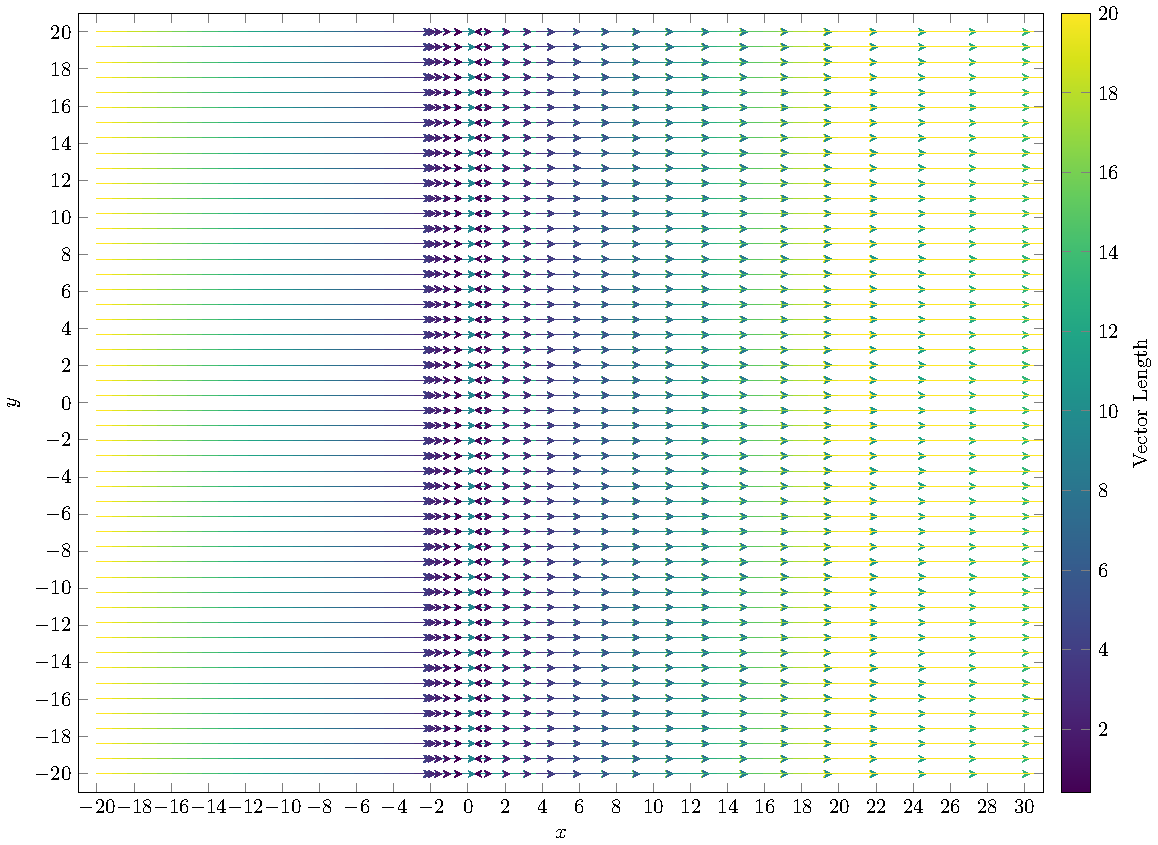
\includegraphics[width=0.75\textwidth]{Figures/VectorSpace1.pdf} 
  \caption{Transition system $(\Z\times\Z, \delta)$ in the interval $[-20,20]\times[-20,20]$. The behaviour of pairs $(x,y)$ preserves the value of $y$. In this diagram and in the following ones, the length of the transition is encoded through the colour.} 
  \label{fig:IntroVectorSpace}
\end{figure} 
\begin{figure}[!t]
  \centering
  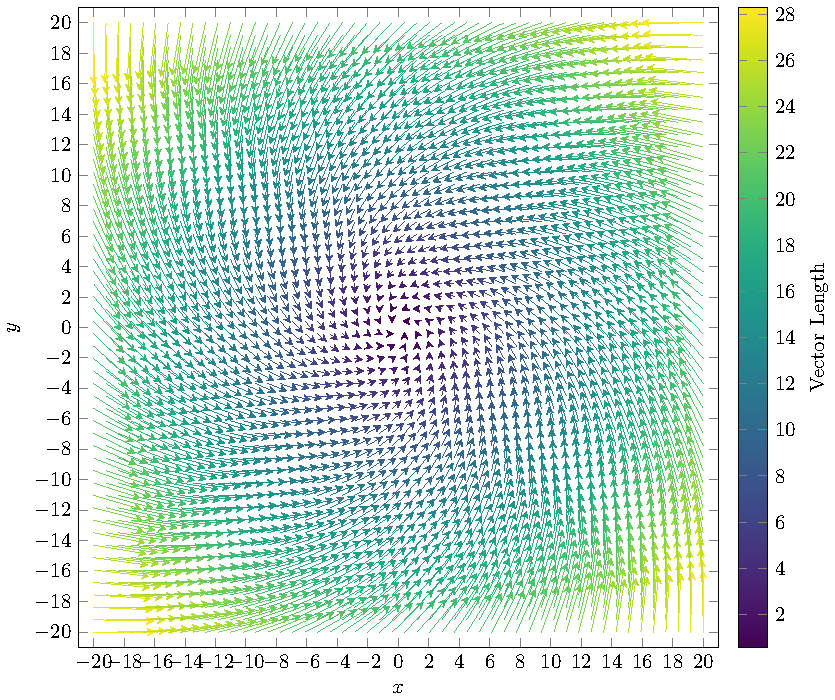
\includegraphics[width=0.75\textwidth]{Figures/VectorSpace2.pdf} 
  \caption{The spatial transformation $m$ as a vector field in the interval $[-20,20]\times[-20,20]$. The function $m$ rotates pairs by 90 degrees counter-clockwise.} 
  \label{fig:SpatialDeformation} 
\end{figure} 

Since $(\Z\times\Z, \delta)$ is the current transition system, we interpret $m$ as a spatial transformation whose application reveals the system shown in Figure~\ref{fig:SecondLatent}. %, where we apply $m$ first and then $\delta$, mapping $(x,y)$ to $(y^2,x)$. 
The behaviour of a pair $(x,y)$ is now very different: the iterated application of the function $\delta\circ m$ returns $(-y,x^2),(-x^2,y^2),(-y^2,x^4)$, etc. Although the behaviour of states in the systems $(\Z\times\Z, \delta)$ and $(\Z\times\Z, \delta\circ m)$ are quite different, their sole difference is the presence of the spatial transformation $m$. 
\begin{figure}[!t]
  \centering
  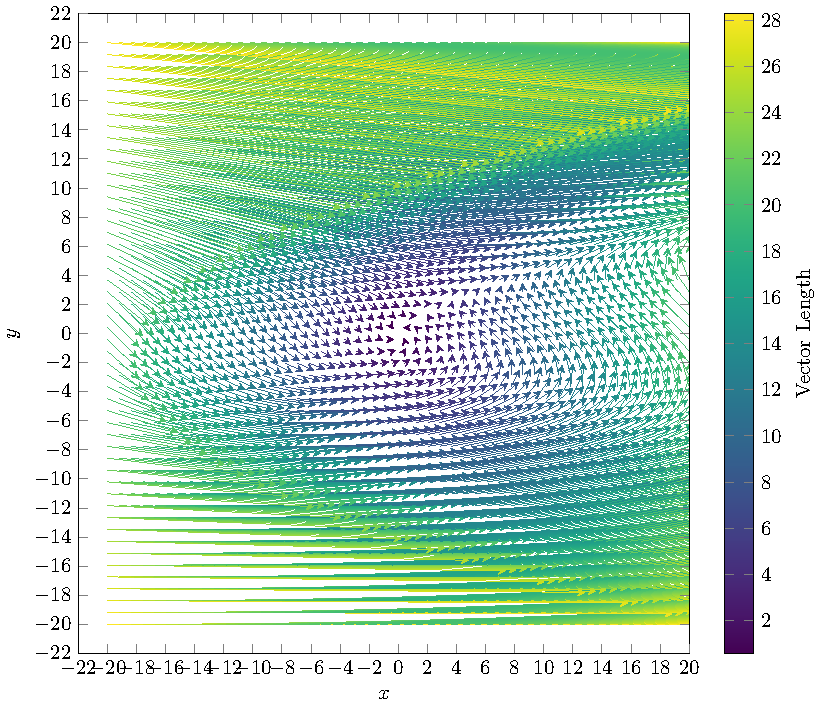
\includegraphics[width=0.75\textwidth]{Figures/VectorSpace4.pdf} 
  \caption{Latent behaviour of $(\Z\times\Z, \delta)$ revealed by the spatial transformation $m$ in the interval $[-20,20]\times[-20,20]$.}
  \label{fig:FirstLatent}
\end{figure} 
\begin{figure}[!t]
  \centering
  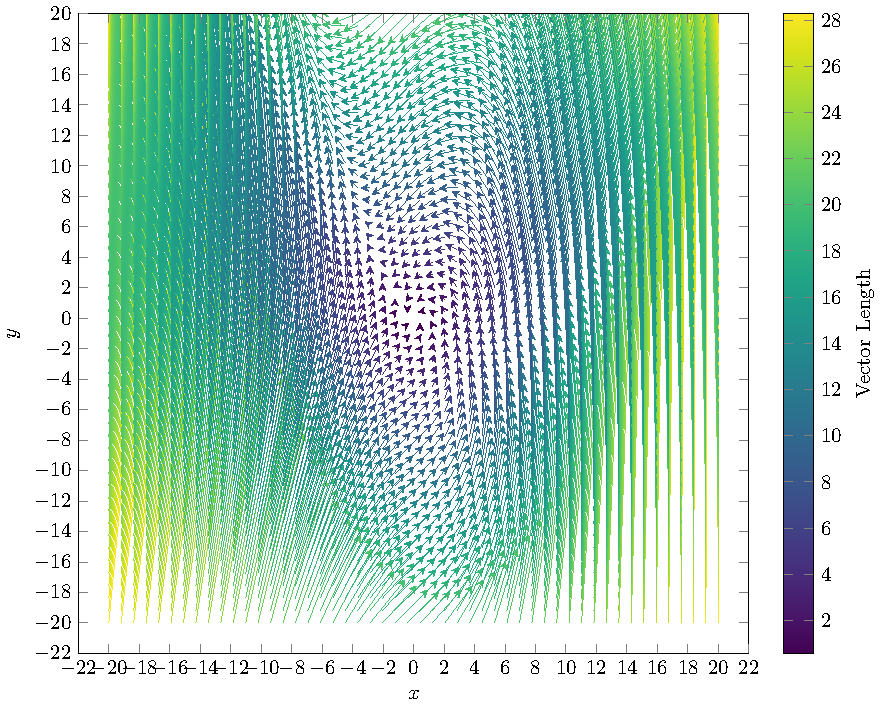
\includegraphics[width=0.75\textwidth]{Figures/VectorSpace3.pdf} 
  \caption{Dual latent behaviour of the system $(\Z\times\Z, m)$ revealed by $\delta$ in the interval $[-20,20]\times[-20,20]$. It is a rotation of the behaviour shown in Figure~\ref{fig:FirstLatent}.}
  \label{fig:SecondLatent} 
\end{figure}

% The transformation $m$ causes the behaviour of the system to lose the behavioural property of preserving the value of $y$ for every pair $(x,y)$.  so if an attacker was capable of applying $m$ to the system $(\Z\times\Z, \delta)$, then they can clearly break the value preservation property. 

%Now, the behaviour of $x\in\Nat$ changes from $x+1,x+2,x+3,x+4,\ldots$ to $2x+1,4x+3,8x+7,16x+15\ldots$. 
%The original system $(\Z\times\Z, \delta)$ not have these behaviours, as they are only revealed after applying $*_2$ by, e.g., an attacker. 
% We can vary the spatial transformation $m\colon \Z\times\Z\rightarrow \Z\times\Z$ to reveal reveals a behaviour that uses the transition function of the system $(\Nat, +_1)$. In the dual case, to apply $+_1$ first and then $*_2$ is equivalent to reveal a new behaviour for the transition system $(\Nat, *_2)$ using $+_1$. These new behaviours are \emph{latent}, since they are only revealed in the presence of a non-trivial spatial transformation. 

In this thesis, we intend to model attackers of a system as sets of spatial transformations. Using these spatial transformations, the attackers cause the system to reveal new behaviours only by affecting the state space, leaving the transition function intact. This implicitly creates a ``game" between attacker and system: the attacker moves first and transforms the initial state, the system then moves by applying its transition function, and then the attacker moves again, transforming the resulting states. The system moves again, and this process iterates. We do not consider cases where the attacker takes two turns in a row or where the system takes two turns in a row, since we can emulate them by an intercalated game. More precisely, an attacker that takes two turns in a row to transform a state $x$ into a state $y$ and then to a state $z$ is equivalent to an attacker that takes only one turn and transforms $x$ into $z$ directly. A system that takes two turns in a row by mapping a state $a$ to a state $b$ and then to a state $c$ is equivalent to a turn-based game between an attacker and system where the attacker used an identity transformation to map $a$ to itself and $b$ to itself. 

An attacker that can only apply an identity spatial transformation (i.e., one that maps a state to itself) has only trivial capabilities, and fits a passive attacker model that can only watch as the system executes. An attacker that can apply any spatial transformations can manipulate the state space of the transition system as they wish, rendering the dynamics of the system obsolete because they can be bypassed via spatial transformations. We define realistic attacker models by imposing restrictions over the spatial transformations that are available to an attacker. % For example, an attacker that can execute the spatial transformation in Figure~\ref{fig:VectorSpace2} is an attacker that can flip the components of the pairs, and negate the first component afterwards.
For example, the attackers described by Basin and Cremers in~\cite{KnowYourEnemy} cannot transform every state of the protocol; they can only transform the states that satisfy the premises of the
%Although this formalism discards attackers that can change the program of the system,  %By protecting the operational semantics of the transition system (i.e., the transition function), we force attackers to follow the rules 
compromise rules available to them, and the transformation must implement the effects modelled by the compromise rule. %An attacker model is a set of compromise rules, so more capable attackers have more enabled transitions at their disposal. We interpret the transitions enabled by the compromise rules as a spatial transformation that reveals latent behaviours. 

Not all systems have their dynamics described in terms of endofunctions. For example, reactive systems require an external inputs to continue execution. To define a unified methodology for the application of spatial transformations in transition systems, we use \emph{universal coalgebra}.


% % Without any restrictions, spatial transformations can map states in any imaginable way.

% From a high-level perspective, we compose the effect of the attacker with the effects of the normal behaviour of the system, and we study the composition to measure robustness and find ways to improve it.

\section{Universal Coalgebra and Spatial Transformations}
To soundly extend the applicability of the ``game" between spatial transformations and deterministic systems to other models of computation, we adopt the framework of \emph{universal coalgebra}~\cite{UniversalCoalgebra}.  
Several authors have used universal coalgebra to generalise results previously exclusive to certain computational models; e.g., the \emph{powerset construction}, a standard procedure to discretise a non-deterministic finite automaton, generalises to other computational effects beyond non-determinism~\cite{GeneralisingDetermination}, or e.g., Kleene's Theorem~\cite{KleenesTheorem}, which states that every deterministic finite automaton has an equivalent regular expression, generalises to Mealy machines~\cite{KleeneCoalgebra}.  

In universal coalgebra, a dynamical system is often represented as a pair $(X,c)$ where $X$ is a set, called the \emph{carrier}, and $c\colon X\rightarrow F(X)$ is a function where $F(X)$, informally, is the set of the features and computational effects that the elements of $X$ may have (e.g., continuation, termination, input/output, etc.). Using the framework of universal coalgebra, our definitions naturally adapt from one computational model to another, widening their applicability. 

% % Brzozowski's algorithm for the minimisation of deterministic finite automata can be generalised to deterministic Moore automata~\cite{CoBrzozowski}.

% We would like our definitions of attacker models to be as general as they possibly can so that they apply to as many systems as possible. For that reason, we model systems and attackers using the . 

% Universal coalgebra has also been used for applications in system security. 

\section{Goal of the Thesis and Outline}
\label{sec:Introduction:Goal}
The main objective of the thesis is to illustrate the usefulness and versatility of parametrising the study of transition systems with a spatial transformation that reveals latent behaviours, a process that we call \emph{latent behaviour analysis} (LBA). These latent behaviours capture extraordinary semantics that are realisable by the systems under the effect of state corruption or alterations; using LBA we can systematically study the behaviour of systems in the presence of adversaries or under the influence of property enforcers. We use universal coalgebra to define LBA in an abstract setting, and we illustrate its applicability in three practical scenarios: the classification of attacker models of a reactive system, the quantification and improvement of robustness in cyber-physical systems (CPS), and the enforcement of timing side-channel freedom in LLVM-IR programs. 

We divide this thesis into two major modules: \emph{theory} and \emph{applications}. The theory module presents LBA in the framework of universal coalgebra (Chapter~\ref{ch:LatentBehaviours}), and the application module shows three different instances of the application of LBA to three practical problems: the classification of attacker models in Chapter~\ref{ch:Classification}, the quantification and repair of robustness in CPS in Chapter~\ref{ch:CPSRobustness}, and the enforcement of timing side-channel freedom with respect to memory access patterns for LLVM-IR programs in Chapter~\ref{ch:SideChannelRepair}.

\section{Research Questions and Summary of Contributions}
\label{sec:Introduction:ResearchQuestions}
To accomplish the goal of this thesis, we study the following research questions. When appropriate, we analyse these questions in the context of the application scenarios for LBA that we present in the following chapters. 
\begin{question}
\label{que:AttackerModel}
How do we precisely and systematically describe and generate attacker models, attacks and attackers?
\end{question}
We approach this question by modelling attacker models with sets of capabilities that create spatial transformations that model the attacks available for attackers fitting that model. We discuss this question in detail in Chapters~\ref{ch:LatentBehaviours},~\ref{ch:Classification}, and~\ref{ch:CPSRobustness}.
\begin{question} 
\label{que:Quantification}
How do we efficiently quantify the harmful effects of an attacker fitting a given attacker model on a system? 
\end{question}
The presence of an attacker does not necessarily imply a security risk, e.g., if the attacker can only slightly deviate the behaviour of the system without breaking any security requirements. To address this question, we propose a quantification method that uses bounded model checking in Chapter~\ref{ch:Classification} and that uses testing in Chapter~\ref{ch:CPSRobustness}. %We implement the systematic quantification of the effect of attackers via LBA. 

\begin{question}
\label{que:Classification}
How do we compare attacker models and attackers concerning the impact that they potentially have on a given system?
\end{question}
Attackers that have more interaction points with a system are not necessarily the most dangerous. We take inspiration from Basin and Cremers~\cite{KnowYourEnemy} to approach this question. To determine which attackers are more threatening, we use the quantification methods proposed in Chapter~\ref{ch:Classification} and Chapter~\ref{ch:CPSRobustness} to obtain a partial order of attackers relative to their harmful effects on systems. In particular, thanks to our modelling of attackers via sets of spatial transformations, the partial order of attackers that naturally arises from set inclusion has a monotonicity property for the harmful effects of attackers on a system. We explain this monotonicity property in Chapters~\ref{ch:Classification} and~\ref{ch:CPSRobustness}.

\begin{question}
\label{que:Repair}
How do we repair a system that is vulnerable to a given attacker model?
\end{question}
Finally, we approach this broad question from two directions: first, we show how LBA can suggest counterattacks for identified attacks in Chapters~\ref{ch:CPSRobustness}, and second, we explain how to use spatial transformations to enforce a security property (i.e., timing side-channel freedom) in Chapter~\ref{ch:SideChannelRepair}. 

% We do not claim to expand beyond the state of the art in coaglebras, instead, our interest lies primarily on applications for which spatial transformations of transition systems provide an insight or a benefit for an application. 


% {\color{blue}
% \subsection{Universal Coalgebra and Security}
% \todo[inline]{Write about kleene coalgebra and other applications }
% \todo[inline]{Heap}


% %; in other words, the attackers can \emph{corrupt} the current state of systems.



% Although the work of Basin and Cremers addresses a confidentiality issue, 

% How do we define realistic attacker models for transition systems? Perhaps it is easier if we start with a system as simple as possible. 
% \todo[inline]{maybe something on fault analysis? I dunno.}


% %If an attacker can arbitrarily change the transition structure of a system, is it possible to defend against such attacker? 
% %It is an idea compatible with both model checking and testing, which is how we can obtain hierarchies of systems. 
% %While Basin and Cremers study the effect of attackers for confidentiality, we are interested in studying the effect of attackers for integrity. Clarkson and Schneider write~\cite{QuantitativeIntegrity} 


% %  span over three dimensions: \emph{which} data is compromised, \emph{whose} data is it, and \emph{when} the compromise occurs. In a nutshell, a they model a protocol 

% % %Attackers that are powerful can replicate the actions of weaker attackers, 

% % Pairing systems and attacker models to obtain a position



% % In particular, \emph{cyber-physical systems} (CPS), which comprise a majority of the critical infrastructure in many countries, 

% % \emph{Universal coalgebra}~\cite{UniversalCoalgebra} 






% \todo[inline]{Biba Duality}
% \todo[inline]{Basin Cremers attackers as sets of effects KYE}
% \todo[inline]{Confidentiality: test if attackers have some knowledge; Integrity: test if the system is too corrupted.}
% \todo[inline]{What, when, how? Modelling attacks}
% \todo[inline]{if we know what attacker models are mathematically, we can ask the computer to do analysis for us in integrity. }
% \todo[inline]{YOU HAVE TO ADDRESS the problem for confidentiality and cite relevant papers, and quantificaiton}
% \todo[inline]{What does Unifying Facets of Information Integrity say?}

% \todo[inline]{The idea is that there is a lot of stuff, but they ultimately belong to a bigger set of ``program correctness''. We argue that those are behavioural properties}

% \todo[inline]{Coalgebras provide a clear view of the set of behavioural properties for families of systems. That makes them really attractive for studying. Not only that, they offer generalised processes for the incorporation of computational effects (e.g., non-determinism, exceptions, termination, etc.) because of category theory.}

% Probably the most important is to motivate the quantification of attackers and how it gave rise to the general treatment of latent behaviours.
% \todo[inline]{}
% \todo[inline]{The first thing we need to do is describe why latent behaviours are interesting. This requires a historical context. }
% \section{Coalgebras}
% \todo[inline]{This section explains the importance of coalgebras as a modelling system, why they are so compatible with computability (monads), and in general why they are useful.}
% \todo[inline]{I could probably be inspired on how to structure this section by publications on coalgebras. There is a large body of literature I can use.}
% \todo[inline]{At least cover that systems are of a form $\delta\colon X\rightarrow D$ where $D$ is some domain, and that there is a way to go from $D$ back to $X$ to continue computation.}
% \todo[inline]{Final coalgebras are important because $D=X$, so it is obvious how to continue.}

% \section{Latent Behaviours}
% \todo[inline]{Explain that in this document we explore the notion of creating new behaviours through transformations of the state space of systems.}
% \subsection{Intuition}
% \todo[inline]{We present a light version of latent behaviours: you normally start at $X$, then you go to $D$ and then back to $X$, but what if we transformed $X$?}
% In latent behaviours we use a transformation $X\rightarrow X$ to affect the behaviour of the system. This transformation is an abstraction; the original system naturally transforms to a system $X\rightarrow D \rightarrow X$ using composition, also of type $X\rightarrow X$. Each function $X\rightarrow X$ can be seen as a black-box of some behaviour. Their interweaving means that they are acting simultaneously. 



% We do not pretend to solve these questions at this broad level, but we address concrete instances of these questions, which appear as we instantiate systems, attacker models, security requirements, etc. in the following sections.
% \section{Applications}
% \subsection{Attacker Classification}
% How can we model attackers? How can we model their actions? How can we prepare against them?
% \subsection{Cyber-Physical System Redesign}
% Many attacks are discovered through testing: an experienced hacker creates a proof of concept to illustrate how some system may be attacked. Then, an abstraction is created to explain why the attack works, and to suggest countermeasures against it. 
% \subsection{Program Repair}



%Fuzzing is probably one of the most popular techniques for system transformations. 

% \todo[inline]{Actually, the thesis would be super interesting if potential behaviour problems are presented in terms of a game between the system and the attacker, with the attacker following some sort of reactive strategy, and the system as well. At some point, one or the other wins because it is a deterministic game if the system is deterministic. }



% \todo[inline]{You can probably show several papers that display this pattern.} 

